%!TEX program = lualatex
% Arquivo: guia_estudos_zoologia_annelida_echinodermata_v01.tex
% Compilar com LuaLaTeX.
% A seção de Lofoforados foi deixada reservada para inserção posterior,
% quando o material da disciplina estiver disponível.

\documentclass[a4paper,12pt]{article}

% =========================================================
% Idioma e tipografia — LuaLaTeX
% =========================================================
\usepackage[brazilian]{babel}
\usepackage{fontspec}
\setmainfont{Latin Modern Roman}
\setsansfont{Latin Modern Sans}
\setmonofont{Latin Modern Mono}
\usepackage{microtype}

% =========================================================
% Página e parágrafos
% =========================================================
\usepackage[
  top=2.8cm,
  bottom=2.5cm,
  left=3cm,
  right=2.5cm
]{geometry}
\usepackage{setspace}
\onehalfspacing
\usepackage{indentfirst}
\setlength{\parindent}{1.25cm}
\setlength{\parskip}{0.15em}

% =========================================================
% Tabelas, listas, caixas e figuras
% =========================================================
\usepackage{booktabs}
\usepackage{tabularx}
\usepackage{longtable}
\usepackage{array}
\usepackage{enumitem}
\usepackage{xcolor}
\usepackage[most]{tcolorbox}
\usepackage{graphicx}
\usepackage{float}
\usepackage{caption}
\usepackage{ragged2e}
\usepackage{amsmath,amssymb}
\usepackage{hyperref}
\usepackage{titlesec}

\hypersetup{
  colorlinks=true,
  linkcolor=blue!45!black,
  urlcolor=blue!50!black,
  pdftitle={Guia de Estudos — Zoologia: Annelida e Echinodermata},
  pdfauthor={Material de estudo}
}

\setlist[itemize]{leftmargin=1.2cm,itemsep=0.25em,topsep=0.25em}
\setlist[enumerate]{leftmargin=1.2cm,itemsep=0.35em,topsep=0.25em}

\newcolumntype{Y}{>{\RaggedRight\arraybackslash}X}
\newcolumntype{P}[1]{>{\RaggedRight\arraybackslash}p{#1}}

\definecolor{corprova}{RGB}{255,247,214}
\definecolor{corpratica}{RGB}{229,243,255}
\definecolor{coratencao}{RGB}{255,230,226}
\definecolor{corconceito}{RGB}{235,247,235}

\newtcolorbox{pontoprova}{
  breakable,
  colback=corprova,
  colframe=orange!60!black,
  title={Ponto de prova},
  fonttitle=\bfseries
}
\newtcolorbox{pratica}{
  breakable,
  colback=corpratica,
  colframe=blue!55!black,
  title={Reconhecimento em aula prática},
  fonttitle=\bfseries
}
\newtcolorbox{atencao}{
  breakable,
  colback=coratencao,
  colframe=red!55!black,
  title={Atenção},
  fonttitle=\bfseries
}
\newtcolorbox{conceito}{
  breakable,
  colback=corconceito,
  colframe=green!45!black,
  title={Conceito-chave},
  fonttitle=\bfseries
}

\titleformat{\section}{\Large\bfseries}{\thesection}{0.7em}{}
\titleformat{\subsection}{\large\bfseries}{\thesubsection}{0.7em}{}
\titleformat{\subsubsection}{\normalsize\bfseries}{\thesubsubsection}{0.7em}{}

\newcommand{\termo}[1]{\textbf{#1}}
\newcommand{\grupo}[1]{\textit{#1}}

\begin{document}

\begin{titlepage}
\centering
\vspace*{2.5cm}
{\Huge\bfseries Guia de Estudos — Zoologia\par}
\vspace{0.8cm}
{\LARGE Lofoforados, Annelida e Echinodermata\par}
\vspace{1.2cm}
{\large Fundamentos de Biologia III\par}
\vfill
\begin{tcolorbox}[colback=gray!5,colframe=gray!45,width=.88\textwidth]
\centering
\textbf{Versão 01 — em construção}\par
\medskip
Nesta versão estão desenvolvidos \textbf{Annelida} e \textbf{Echinodermata}. A parte de \textbf{Lofoforados} está reservada para ser incorporada depois, a partir do material específico da disciplina.
\end{tcolorbox}
\vfill
{\large Material preparado a partir das aulas teóricas, roteiros práticos e fotografias fornecidas para estudo.\par}
\end{titlepage}

\tableofcontents
\newpage

% =========================================================
\section{Como usar este guia}
% =========================================================

Este texto foi organizado para revisão de prova. A prioridade é ligar quatro níveis de informação:

\begin{enumerate}
  \item \textbf{característica do grupo};
  \item \textbf{estrutura anatômica};
  \item \textbf{função};
  \item \textbf{reconhecimento em material prático}.
\end{enumerate}

Ao estudar cada grupo, tente responder sempre: \emph{``o que eu reconheço?'', ``como diferencio?'', ``qual é a função desta estrutura?'' e ``qual característica é exclusiva ou especialmente importante?''}

\begin{atencao}
Números de espécies e alguns detalhes classificatórios aparecem nos slides porque podem ser cobrados, mas não devem substituir a compreensão das características morfológicas e funcionais.
\end{atencao}

% =========================================================
\section{Lofoforados — seção reservada}
% =========================================================

\begin{tcolorbox}[breakable,colback=gray!6,colframe=gray!50,title={Conteúdo a incorporar}]
Esta seção será preenchida quando o material da aula de Lofoforados estiver disponível. A inserção deverá preservar a sequência deste guia e incluir: definição e função do lofóforo; organização corporal; alimentação; grupos apresentados em aula; comparação entre eles; e reconhecimento prático.
\end{tcolorbox}

\newpage

% =========================================================
\section{Filo Annelida}
% =========================================================

\subsection{Visão geral}

O nome \termo{Annelida} refere-se à aparência anelada do corpo. O material da disciplina destaca como característica central a \termo{segmentação}, associada à grande diversificação do grupo. Os anelídeos estudados incluem os poliquetas e os clitelados, estes últimos representados por oligoquetas e hirudíneos.

\begin{itemize}
  \item corpo segmentado em anéis;
  \item três regiões corporais gerais: \termo{prostômio}, \termo{tronco} e \termo{pigídio};
  \item parede corporal com cutícula fibrosa, epiderme glandular, tecido conjuntivo dérmico e musculatura;
  \item presença de cerdas em muitos representantes;
  \item celoma associado à segmentação e ao funcionamento como esqueleto hidrostático;
  \item sistema nervoso com cérebro anterior dorsal e cordões nervosos longitudinais;
  \item sistema digestório, em condição geral, organizado como tubo da boca ao ânus.
\end{itemize}

\begin{conceito}
A segmentação não é apenas uma sequência de ``marcas'' externas. Nos anelídeos típicos, ela está relacionada à repetição interna de compartimentos e estruturas. O material da disciplina destaca como vantagem seletiva uma \textbf{escavação mais eficiente}.
\end{conceito}

\subsection{Regiões do corpo}

\begin{description}[style=nextline,leftmargin=1.0cm]
  \item[Prostômio] Região anterior, associada à cabeça e, em muitos poliquetas, portadora de estruturas sensoriais.
  \item[Tronco] Região segmentada que contém a maior parte dos metâmeros.
  \item[Pigídio] Região terminal posterior; em poliquetas pode apresentar cirros anais.
  \item[Peristômio] Região associada à boca. No roteiro prático de nereidídeos, os primeiros segmentos após o prostômio formam o peristômio ou segmento bucal.
\end{description}

\begin{pontoprova}
\textbf{Prostômio e pigídio não devem ser confundidos com um segmento típico do tronco.} Em perguntas de morfologia externa, identifique primeiro a extremidade anterior, a boca/peristômio e a extremidade posterior; só depois conte ou compare os metâmeros.
\end{pontoprova}

\subsection{Cerdas}

As cerdas dos anelídeos são descritas no material como estruturas de \termo{$\beta$-quitina}, macias e flexíveis, em contraste com a $\alpha$-quitina dura e inflexível citada para artrópodes. O número, posição e forma das cerdas variam muito entre os grupos e são particularmente importantes em Polychaeta.

\subsection{Celoma e esqueleto hidrostático}

O plano corporal apresentado para Annelida inclui um par de cavidades celômicas por segmento, revestidas por mesotélio. Mesentérios dorsal e ventral aparecem associados à organização dessas cavidades. O fluido celômico e a musculatura corporal participam do \termo{esqueleto hidrostático}.

\begin{conceito}
No esqueleto hidrostático, a musculatura atua contra um fluido praticamente incompressível. Assim, a alteração da forma do segmento pode produzir alongamento, encurtamento e deslocamento do corpo sem necessidade de um esqueleto rígido.
\end{conceito}

\subsection{Sistema nervoso e percepção}

O material geral de Annelida descreve:

\begin{itemize}
  \item cérebro anterior e dorsal;
  \item um par de cordões nervosos;
  \item axônios gigantes em alguns representantes;
  \item fotorreceptores, quimiorreceptores e mecanorreceptores associados principalmente ao prostômio e aos apêndices;
  \item em Polychaeta, ocelos, olhos e órgãos nucais;
  \item olhos também podem ocorrer em alguns Hirudinea.
\end{itemize}

\subsection{Circulação e trocas gasosas}

O sistema sanguíneo geral é descrito como \termo{fechado}, com vasos dorsal e ventral, podendo estar reduzido ou ausente em alguns representantes. O material menciona regiões contráteis chamadas, de forma didática, de ``corações'' e a presença de hemoglobina como pigmento respiratório.

As trocas gasosas podem ocorrer:

\begin{itemize}
  \item pela superfície corporal;
  \item por apêndices;
  \item por brânquias, quando presentes.
\end{itemize}

\subsection{Excreção}

A excreção é realizada por \termo{nefrídios}, geralmente organizados em pares segmentares. O material distingue:

\begin{itemize}
  \item \termo{protonefrídios}, associados às formas sem sistema hemal;
  \item \termo{metanefrídios}, associados às formas com sistema hemal.
\end{itemize}

\subsection{Sistema digestório}

A organização geral apresentada é:

\begin{center}
\textbf{boca $\rightarrow$ faringe $\rightarrow$ esôfago $\rightarrow$ estômago $\rightarrow$ intestino $\rightarrow$ ânus}
\end{center}

As especializações variam conforme o hábito alimentar e serão retomadas em cada grupo.

\subsection{Reprodução e desenvolvimento}

O material mostra grande diversidade reprodutiva em Annelida:

\begin{itemize}
  \item reprodução assexuada por fragmentação, brotamento e fissão transversal;
  \item reprodução sexuada;
  \item formas gonocóricas ou hermafroditas;
  \item gônadas dispersas no celoma ou restritas a determinados segmentos;
  \item fecundação externa ou interna;
  \item desenvolvimento indireto, com larva trocófora, ou desenvolvimento direto.
\end{itemize}

% =========================================================
\section{Polychaeta}
% =========================================================

\subsection{Características gerais}

O nome Polychaeta deriva da ideia de ``muitas cerdas''. Os poliquetas apresentados na disciplina são predominantemente marinhos e ocupam diversos modos de vida: bentônicos, cavadores, rastejadores, perfuradores, pelágicos e tubícolas.

A estrutura mais importante para reconhecer o grupo é o \termo{parapódio}. Em condição típica, ocorre um par de parapódios por segmento.

\subsection{Parapódios}

Os parapódios podem ser:

\begin{itemize}
  \item \termo{unirremes};
  \item \termo{birremes}, com ramo dorsal chamado \termo{notopódio} e ramo ventral chamado \termo{neuropódio}.
\end{itemize}

No roteiro prático, cada ramo pode apresentar lígulas e lobos, sacos setígeros e numerosas cerdas. Uma estrutura interna de sustentação, o \termo{acículo}, pode ocorrer no interior dos ramos parapodiais.

\begin{pratica}
Em um parapódio birreme, procure primeiro dois ramos: \textbf{notopódio} dorsal e \textbf{neuropódio} ventral. Depois procure cirros, cerdas e o acículo. O segmento que possui cerdas é chamado \textbf{setígero}.
\end{pratica}

\subsection{Poliquetas errantes — exemplo de Nereididae}

O roteiro prático descreve os poliquetas errantes como formas com numerosos metâmeros geralmente semelhantes, nos quais a segmentação externa corresponde à interna. Em nereidídeos, devem ser reconhecidos:

\begin{itemize}
  \item prostômio;
  \item antenas laterais curtas;
  \item dois pares de olhos;
  \item palpos robustos;
  \item peristômio ou segmento bucal;
  \item cirros tentaculares ou peristomiais;
  \item faringe ou probóscide eversível;
  \item paragnatas quitinosas;
  \item mandíbulas fortes e denteadas;
  \item parapódios com notopódio e neuropódio;
  \item cirros dorsal e ventral;
  \item pigídio, frequentemente com cirros anais.
\end{itemize}

\begin{pontoprova}
\textbf{Nereididae:} a associação ``cabeça bem diferenciada + olhos/palpos/antenas + probóscide eversível + mandíbulas/paragnatas + parapódios desenvolvidos'' é muito mais útil para reconhecimento do que decorar uma única estrutura isolada.
\end{pontoprova}

\subsection{Cerdas em Nereididae}

O roteiro prático destaca cerdas compostas \termo{espinígeras} e \termo{falcígeras}. O acículo não é uma cerda externa de locomoção: ele está inserido no parapódio e atua na sustentação.

\subsection{Poliquetas tubícolas — exemplo de Sabellidae}

Nos poliquetas tubícolas há tendência à especialização de regiões corporais. No material de Sabellidae:

\begin{itemize}
  \item parapódios são reduzidos;
  \item acículo está ausente;
  \item os animais vivem em tubos de areia ou lodo e raramente saem deles;
  \item prostômio reduzido e fundido ao peristômio;
  \item formação de uma \termo{coroa tentacular};
  \item presença de \termo{colar peristomial};
  \item coroa formada por \termo{radíolos};
  \item radíolos podem apresentar \termo{pínulas}, \termo{estilódios} e manchas ocelares;
  \item cerdas torácicas podem ser limbadas ou em ``pioche'';
  \item presença de \termo{uncini}, pequenas estruturas quitinosas denteadas.
\end{itemize}

Na região torácica, as cerdas limbadas são notopodiais e os uncini são neuropodiais; na região abdominal, a posição se inverte. Os uncini auxiliam a fixação do animal à parede do tubo.

\begin{atencao}
\textbf{Coroa tentacular de Sabellidae não é, por si só, ``lofóforo''.} No guia, a terminologia será mantida conforme o roteiro prático: coroa tentacular formada por radíolos. A comparação com Lofoforados será feita somente quando o material específico dessa aula for incorporado.
\end{atencao}

\subsection{Alimentação em Polychaeta}

O material apresenta quatro grandes estratégias:

\begin{itemize}
  \item comedores de depósitos ou detritos;
  \item suspensívoros;
  \item predadores;
  \item parasitas.
\end{itemize}

Entre predadores errantes, o material cita formas com faringe evertida, mandíbulas e, em alguns casos, dentes e glândulas de veneno.

\subsection{Reprodução em Polychaeta}

Além da reprodução assexuada por brotamento ou fissão transversal, o material destaca reprodução sexuada e fenômenos de \termo{epitoquia} e \termo{enxameamento}. A regeneração de tentáculos, palpos, pigídio e prostômio é mencionada, sendo mais intensa em formas errantes.

\subsection{Quadro de reconhecimento — Nereididae e Sabellidae}

\begin{longtable}{P{3.3cm}P{5.2cm}P{5.2cm}}
\toprule
\textbf{Característica} & \textbf{Nereididae / errante} & \textbf{Sabellidae / tubícola} \\
\midrule
\endfirsthead
\toprule
\textbf{Característica} & \textbf{Nereididae / errante} & \textbf{Sabellidae / tubícola} \\
\midrule
\endhead
Modo de vida & Errante; locomoção ativa & Vive em tubo; pouco sai do tubo \\
Cabeça & Prostômio evidente, palpos, antenas, olhos & Prostômio reduzido e fundido ao peristômio \\
Estrutura anterior marcante & Probóscide/faringe eversível, mandíbulas e paragnatas & Coroa tentacular com radíolos \\
Parapódios & Bem desenvolvidos & Reduzidos \\
Acículo & Presente no exemplo estudado & Ausente no exemplo estudado \\
Cerdas & Diversas; espinígeras e falcígeras no roteiro & Limbadas, em ``pioche'' e uncini \\
Função de fixação & Parapódios e cerdas participam do deslocamento & Uncini auxiliam a agarrar a parede do tubo \\
\bottomrule
\end{longtable}

% =========================================================
\section{Clitellata}
% =========================================================

\subsection{Características compartilhadas}

O material reúne minhocas e sanguessugas na classe Clitellata e destaca:

\begin{itemize}
  \item ausência de parapódios;
  \item ausência de apêndices cefálicos e pigidiais;
  \item presença de \termo{clitelo};
  \item hermafroditismo com cópula;
  \item desenvolvimento direto.
\end{itemize}

O clitelo está associado a três funções enfatizadas na aula:

\begin{enumerate}
  \item secreção de muco durante a cópula;
  \item produção de albumina para nutrição dos ovos;
  \item formação do casulo que contém ovos e albumina.
\end{enumerate}

% =========================================================
\section{Oligochaeta}
% =========================================================

\subsection{Morfologia externa}

Oligochaeta significa ``poucas cerdas''. O material destaca:

\begin{itemize}
  \item prostômio e pigídio sem apêndices;
  \item ausência de parapódios;
  \item quatro feixes de cerdas por segmento;
  \item cerdas simples e não articuladas;
  \item presença do clitelo em indivíduos sexualmente maduros.
\end{itemize}

\subsection{Locomoção}

A locomoção típica ocorre por movimentos peristálticos associados às cerdas e ao esqueleto hidrostático. O roteiro diferencia o papel da musculatura:

\begin{itemize}
  \item musculatura circular: associada ao alongamento e a cerdas recolhidas;
  \item musculatura longitudinal: associada ao encurtamento e a cerdas protraídas.
\end{itemize}

\subsection{Sistema nervoso e sentidos}

No material, o cérebro encontra-se deslocado posteriormente em relação à condição geral dos anelídeos; em Lumbricidae é indicado no segmento 3. Os dois cordões nervosos estão fundidos. Olhos estão ausentes, mas podem ocorrer ocelos simples, fotorreceptores no tegumento e quimiorreceptores concentrados especialmente no prostômio.

\subsection{Alimentação e digestão}

A maioria é apresentada como depositívora, ingerindo matéria orgânica presente em lama ou solo. Também há detritívoros e espécies aquáticas com outras estratégias.

A sequência digestiva estudada é:

\begin{center}
\textbf{boca $\rightarrow$ faringe $\rightarrow$ esôfago $\rightarrow$ papo $\rightarrow$ moela $\rightarrow$ intestino $\rightarrow$ ânus}
\end{center}

O \termo{papo} participa do armazenamento; a \termo{moela}, da trituração; a \termo{tiflossole} aumenta a superfície associada à absorção intestinal.

\subsection{Circulação, respiração e excreção}

O sangue é impulsionado por vasos contráteis chamados, didaticamente, de ``corações''. O número varia entre os grupos. As trocas gasosas ocorrem principalmente por difusão através da parede corporal; em algumas formas aquáticas podem existir estruturas branquiais. A excreção ocorre por metanefrídios, tipicamente um par por segmento.

\subsection{Reprodução}

Oligoquetas são hermafroditas. Na cópula ocorre transferência mútua de espermatozoides. O clitelo forma o casulo alguns dias depois; o casulo contém albumina. A fecundação é descrita como externa, porém ocorrendo \textbf{dentro do casulo}, e o desenvolvimento é direto.

\begin{pontoprova}
Não confunda ``fecundação externa'' com ``desenvolvimento indireto''. No exemplo da minhoca, a fecundação ocorre no casulo e o desenvolvimento é \textbf{direto}, sem uma larva trocófora livre.
\end{pontoprova}

\subsection{Prática: \textit{Amynthas hawayanus}}

O roteiro prático fornece pontos muito específicos para o exemplar estudado:

\begin{itemize}
  \item observar o deslocamento peristáltico e o esqueleto hidrostático;
  \item dorso mais pigmentado e ventre mais claro;
  \item identificar prostômio, boca e peristômio;
  \item contar os segmentos após o peristômio;
  \item clitelo nos segmentos XIV--XVI;
  \item gonóporos masculinos no segmento XVIII;
  \item gonóporo feminino ímpar no clitelo;
  \item espermatecas entre os segmentos V--VIII;
  \item vaso sanguíneo dorsal visível por transparência;
  \item no exemplar do roteiro, dois pares de corações na altura dos segmentos XII--XIII.
\end{itemize}

% =========================================================
\section{Hirudinoidea / Hirudinomorpha}
% =========================================================

\subsection{Características gerais}

As sanguessugas são apresentadas como o grupo mais especializado entre os clitelados estudados. Compartilham com os oligoquetas ausência de parapódios, ausência de apêndices cefálicos, hermafroditismo, clitelo/casulo e desenvolvimento direto.

Entretanto, apresentam modificações marcantes:

\begin{itemize}
  \item corpo achatado dorsoventralmente;
  \item extremidade anterior afilada;
  \item ventosa anterior e ventosa posterior;
  \item ventosa anterior circundando a boca;
  \item segmentação reduzida e número relativamente fixo de segmentos;
  \item anelações externas secundárias;
  \item cerdas ausentes na maioria das formas;
  \item celoma reduzido e septos ausentes em sanguessugas típicas.
\end{itemize}

\begin{conceito}
As muitas anelações visíveis externamente não devem ser automaticamente contadas como segmentos verdadeiros. O material chama atenção para \textbf{anelações secundárias} e para um número fixo de segmentos em Hirudinoidea.
\end{conceito}

\subsection{Locomoção}

Sanguessugas rastejam ou nadam. O material ressalta que elas não escavam usando o peristaltismo típico das minhocas. A locomoção pode envolver alternância de fixação pelas ventosas, produzindo movimento semelhante ao de um ``mede-palmos''.

\subsection{Trocas gasosas e excreção}

As trocas gasosas podem ocorrer pela epiderme e, em alguns grupos, por brânquias. O sistema excretor apresenta de 10 a 17 pares de metanefrídios no material estudado, com papel importante na osmorregulação.

\subsection{Alimentação e sistema digestório}

O material distingue formas hematófagas e predadoras. Entre as hematófagas, a secreção de \termo{hirudina}, um anticoagulante produzido por glândulas salivares, é uma característica importante.

A sequência digestiva apresentada é:

\begin{center}
\textbf{boca $\rightarrow$ faringe $\rightarrow$ esôfago $\rightarrow$ estômago $\rightarrow$ intestino $\rightarrow$ ânus}
\end{center}

A digestão dos hematófagos é muito lenta e depende de microbiota mutualística.

\subsection{Reprodução}

O material destaca reprodução sexuada, hermafroditismo protândrico e fecundação interna. Em alguns grupos ocorre transferência direta pelo aparelho copulador; em outros, transferência por impregnação hipodérmica. Após a cópula, o clitelo torna-se evidente e secreta o casulo.

O desenvolvimento é direto na maioria; algumas formas apresentam cuidado parental, com casulos ou juvenis associados ao ventre da mãe.

\subsection{Prática: reconhecimento de uma sanguessuga}

No roteiro prático, devem ser identificados:

\begin{itemize}
  \item ventosa anterior;
  \item ventosa posterior;
  \item boca;
  \item segmentos;
  \item ocelos, quando presentes;
  \item região clitelar;
  \item anelações secundárias;
  \item abertura anal;
  \item poros genitais masculino e feminino.
\end{itemize}

\IfFileExists{imagens/hirudinea_exemplar.jpg}{
\begin{figure}[H]
  \centering
  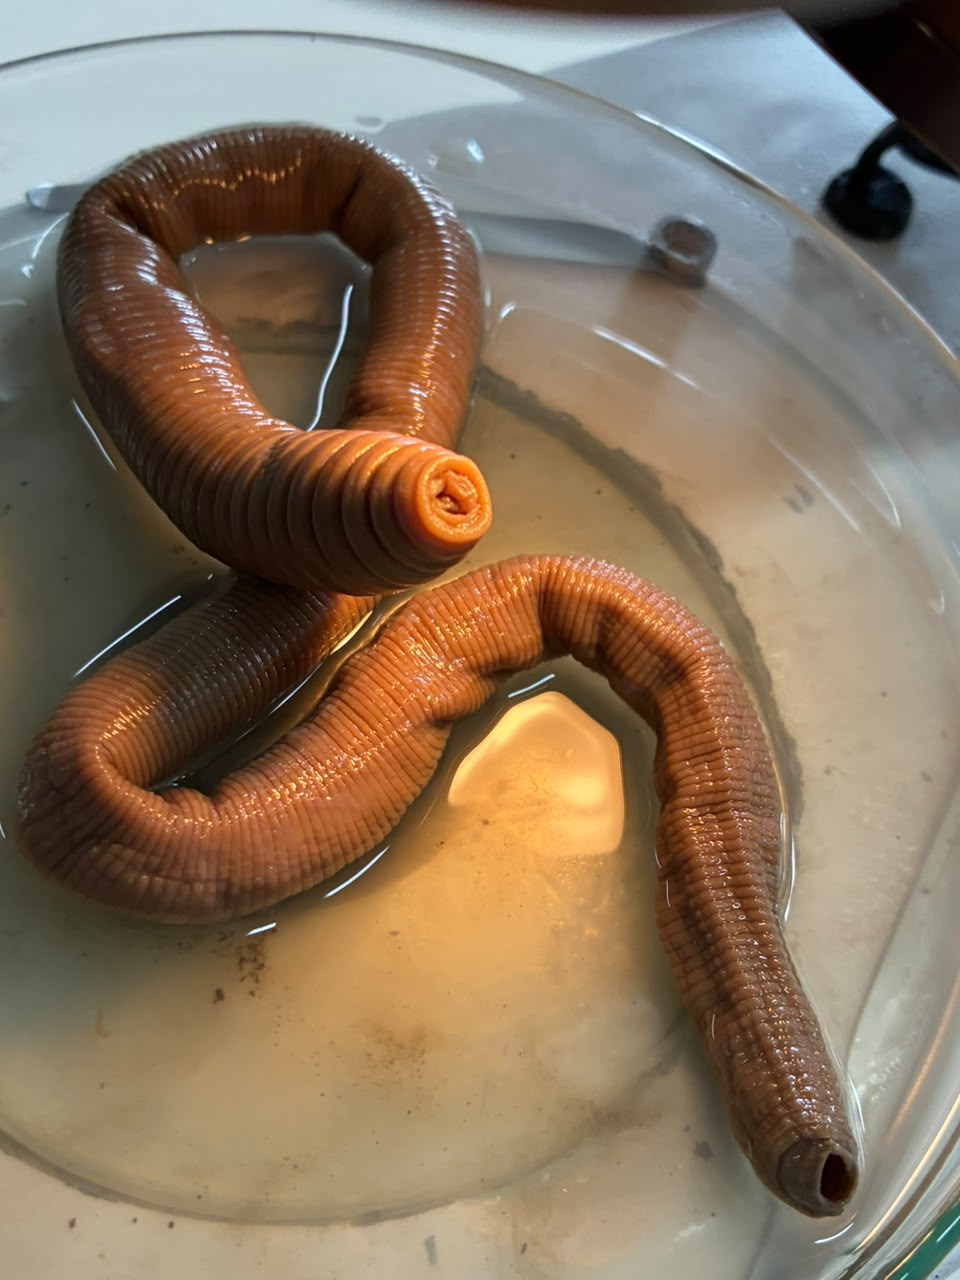
\includegraphics[width=.66\linewidth]{imagens/hirudinea_exemplar.jpg}
  \caption{Material fotográfico de aula: exemplar compatível com Hirudinoidea, útil para observar a forte anelação externa e as extremidades modificadas em ventosas. A identificação taxonômica em nível de espécie não é feita aqui.}
  \label{fig:hirudinea-exemplar}
\end{figure}
}{}

\IfFileExists{imagens/hirudinea_ventosa_detalhe.jpg}{
\begin{figure}[H]
  \centering
  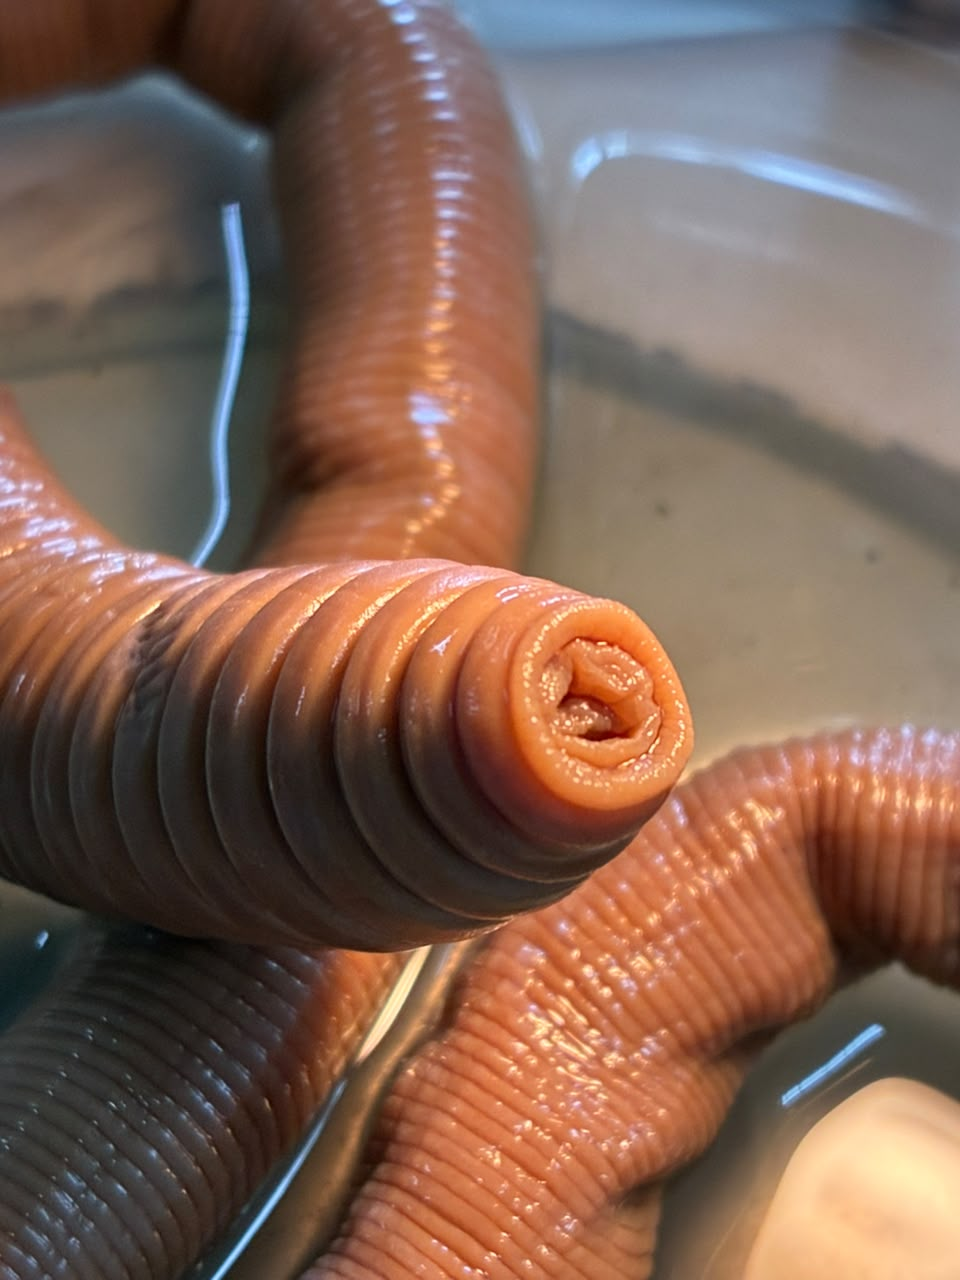
\includegraphics[width=.62\linewidth]{imagens/hirudinea_ventosa_detalhe.jpg}
  \caption{Detalhe de uma das extremidades do exemplar, evidenciando a estrutura em ventosa.}
  \label{fig:hirudinea-ventosa}
\end{figure}
}{}

% =========================================================
\section{Comparação: Polychaeta, Oligochaeta e Hirudinoidea}
% =========================================================

\begin{longtable}{P{3.2cm}P{3.7cm}P{3.7cm}P{3.7cm}}
\toprule
\textbf{Característica} & \textbf{Polychaeta} & \textbf{Oligochaeta} & \textbf{Hirudinoidea} \\
\midrule
\endfirsthead
\toprule
\textbf{Característica} & \textbf{Polychaeta} & \textbf{Oligochaeta} & \textbf{Hirudinoidea} \\
\midrule
\endhead
Parapódios & Presentes em condição típica & Ausentes & Ausentes \\
Cerdas & Muitas e muito variadas & Poucas, simples & Ausentes na maioria \\
Apêndices cefálicos & Frequentemente desenvolvidos & Ausentes & Ausentes \\
Clitelo & Não é característica do grupo & Presente & Presente, podendo ser pouco evidente fora do período reprodutivo \\
Locomoção & Parapódios, musculatura e cerdas; varia conforme modo de vida & Peristaltismo + cerdas + esqueleto hidrostático & Rastejamento/natação; ventosas importantes \\
Celoma/septos & Segmentação celômica bem desenvolvida na condição geral & Esqueleto hidrostático segmentado & Celoma reduzido e septos ausentes nas sanguessugas típicas \\
Reprodução & Sexuada e assexuada; larva pode ocorrer & Hermafroditas; casulo; desenvolvimento direto & Hermafroditas; casulo; desenvolvimento direto \\
Estrutura marcante em prática & Parapódios, cerdas, cabeça ou coroa tentacular & Clitelo e poucas cerdas & Ventosas e anelações secundárias \\
\bottomrule
\end{longtable}

\newpage

% =========================================================
\section{Filo Echinodermata}
% =========================================================

\subsection{Visão geral}

Echinodermata é um filo exclusivamente marinho. O nome deriva de \emph{echinos}, ``espinho'', e \emph{derma}, ``pele''. O material da disciplina destaca ocorrência desde a região entremarés até grandes profundidades e um registro fóssil muito antigo, conhecido desde o Cambriano.

As características centrais trabalhadas em aula são:

\begin{itemize}
  \item condição deuterostômia;
  \item larvas bilateralmente simétricas;
  \item adultos com simetria radial pentâmera derivada;
  \item eixo corporal oral--aboral;
  \item endoesqueleto calcário de origem mesodérmica;
  \item estereoma;
  \item sistema ambulacral ou hidrovascular;
  \item ausência de órgãos excretores;
  \item grande capacidade de autotomia e regeneração em vários grupos.
\end{itemize}

\subsection{Deuterostomia e simetria}

O material compara protostômios e deuterostômios e apresenta Echinodermata como deuterostômio. Na comparação embrionária mostrada em aula, o blastóporo origina o ânus e a clivagem é radial.

Os equinodermos apresentam uma mudança importante ao longo do desenvolvimento:

\begin{center}
\textbf{larva: simetria bilateral $\longrightarrow$ adulto: simetria radial pentâmera}
\end{center}

A simetria pentarradial é, portanto, \textbf{secundária/derivada}. A orientação do corpo adulto utiliza o eixo \termo{oral--aboral}, e não uma distinção simples entre anterior e posterior.

\begin{pontoprova}
Uma estrela-do-mar adulta não representa a condição bilateral ancestral. A bilateralidade aparece claramente nas larvas; a pentarradialidade do adulto foi adquirida posteriormente na evolução do grupo.
\end{pontoprova}

\subsection{Endoesqueleto e estereoma}

O endoesqueleto é de origem mesodérmica e composição calcária. O material descreve placas e ossículos organizados numa rede porosa denominada \termo{estereoma}. A expressão do esqueleto varia muito:

\begin{itemize}
  \item em equinoides, ossículos firmemente fundidos formam uma carapaça rígida ou \termo{testa};
  \item em holotúrias, o esqueleto está reduzido a pequenos ossículos isolados na derme;
  \item em estrelas-do-mar, há numerosos ossículos individuais, numa condição intermediária.
\end{itemize}

O material também menciona tecido colagenoso mutável, capaz de alterar rapidamente a rigidez corporal.

\subsection{Sistema ambulacral ou hidrovascular}

Este sistema é apresentado como característica única dos equinodermos e funciona hidraulicamente. Sua organização geral pode ser memorizada na sequência:

\begin{center}
\textbf{madreporito $\rightarrow$ canal pétreo $\rightarrow$ canal circular $\rightarrow$ canais radiais $\rightarrow$ ampolas $\rightarrow$ pés ambulacrais}
\end{center}

As ampolas e os pés ambulacrais são estruturas musculares. A contração da ampola desloca fluido para o pé, promovendo seu alongamento; a contração da musculatura do pé participa da retração.

\begin{conceito}
Os pés ambulacrais não servem apenas para ``andar''. Dependendo do grupo, participam de locomoção, fixação, manipulação/captura de alimento, percepção e trocas gasosas.
\end{conceito}

\subsection{Sistema nervoso, circulação, respiração e excreção}

O sistema nervoso é descrito com anel circum-oral e nervos radiais, sem cérebro. Há poucos órgãos sensoriais altamente especializados.

A circulação não corresponde a um sistema sanguíneo típico como em vertebrados. O material destaca a circulação celômica e o sistema hemal, cuja função inclui distribuição de nutrientes absorvidos pelo trato digestivo.

A respiração varia entre as classes e pode envolver:

\begin{itemize}
  \item pápulas;
  \item pés tubulares;
  \item bursas em ofiuroides;
  \item árvore respiratória em holoturoides.
\end{itemize}

Órgãos excretores estão ausentes.

\subsection{Reprodução e regeneração}

O material apresenta sexos separados na maioria das espécies, raros hermafroditas, fecundação geralmente externa e desenvolvimento com estágios larvais na maioria, embora haja desenvolvimento direto em alguns grupos.

Também são destacados:

\begin{itemize}
  \item autotomia;
  \item regeneração de partes perdidas;
  \item reprodução assexuada por fissiparidade em representantes de Asteroidea, Ophiuroidea e Holothuroidea.
\end{itemize}

% =========================================================
\section{As cinco classes de Echinodermata}
% =========================================================

\subsection{Crinoidea — lírios-do-mar}

Características apresentadas no material:

\begin{itemize}
  \item corpo em forma de taça;
  \item superfície oral voltada para cima;
  \item região aboral com pedúnculo ou cirros;
  \item braços com pínulas;
  \item braços e ambúlacros podem ramificar-se;
  \item madreporito ausente;
  \item boca e ânus na superfície oral.
\end{itemize}

Quanto à alimentação, o material complementar caracteriza crinoides como consumidores de plâncton e partículas em suspensão.

\subsection{Asteroidea — estrelas-do-mar}

Características diagnósticas:

\begin{itemize}
  \item corpo estrelado com cinco ou mais braços;
  \item braços surgem gradualmente do disco central, sem separação/articulação nítida;
  \item boca voltada para o substrato;
  \item ânus na face aboral;
  \item madreporito aboral;
  \item sulcos ambulacrais abertos;
  \item pés ambulacrais com ou sem ventosas;
  \item pápulas dérmicas;
  \item pódios sensoriais na ponta dos braços em exemplos apresentados.
\end{itemize}

A maioria é apresentada como predadora carnívora; o material complementar destaca a capacidade de eversão do estômago em estrelas-do-mar.

\IfFileExists{imagens/asteroidea_face_oral.jpg}{
\begin{figure}[H]
  \centering
  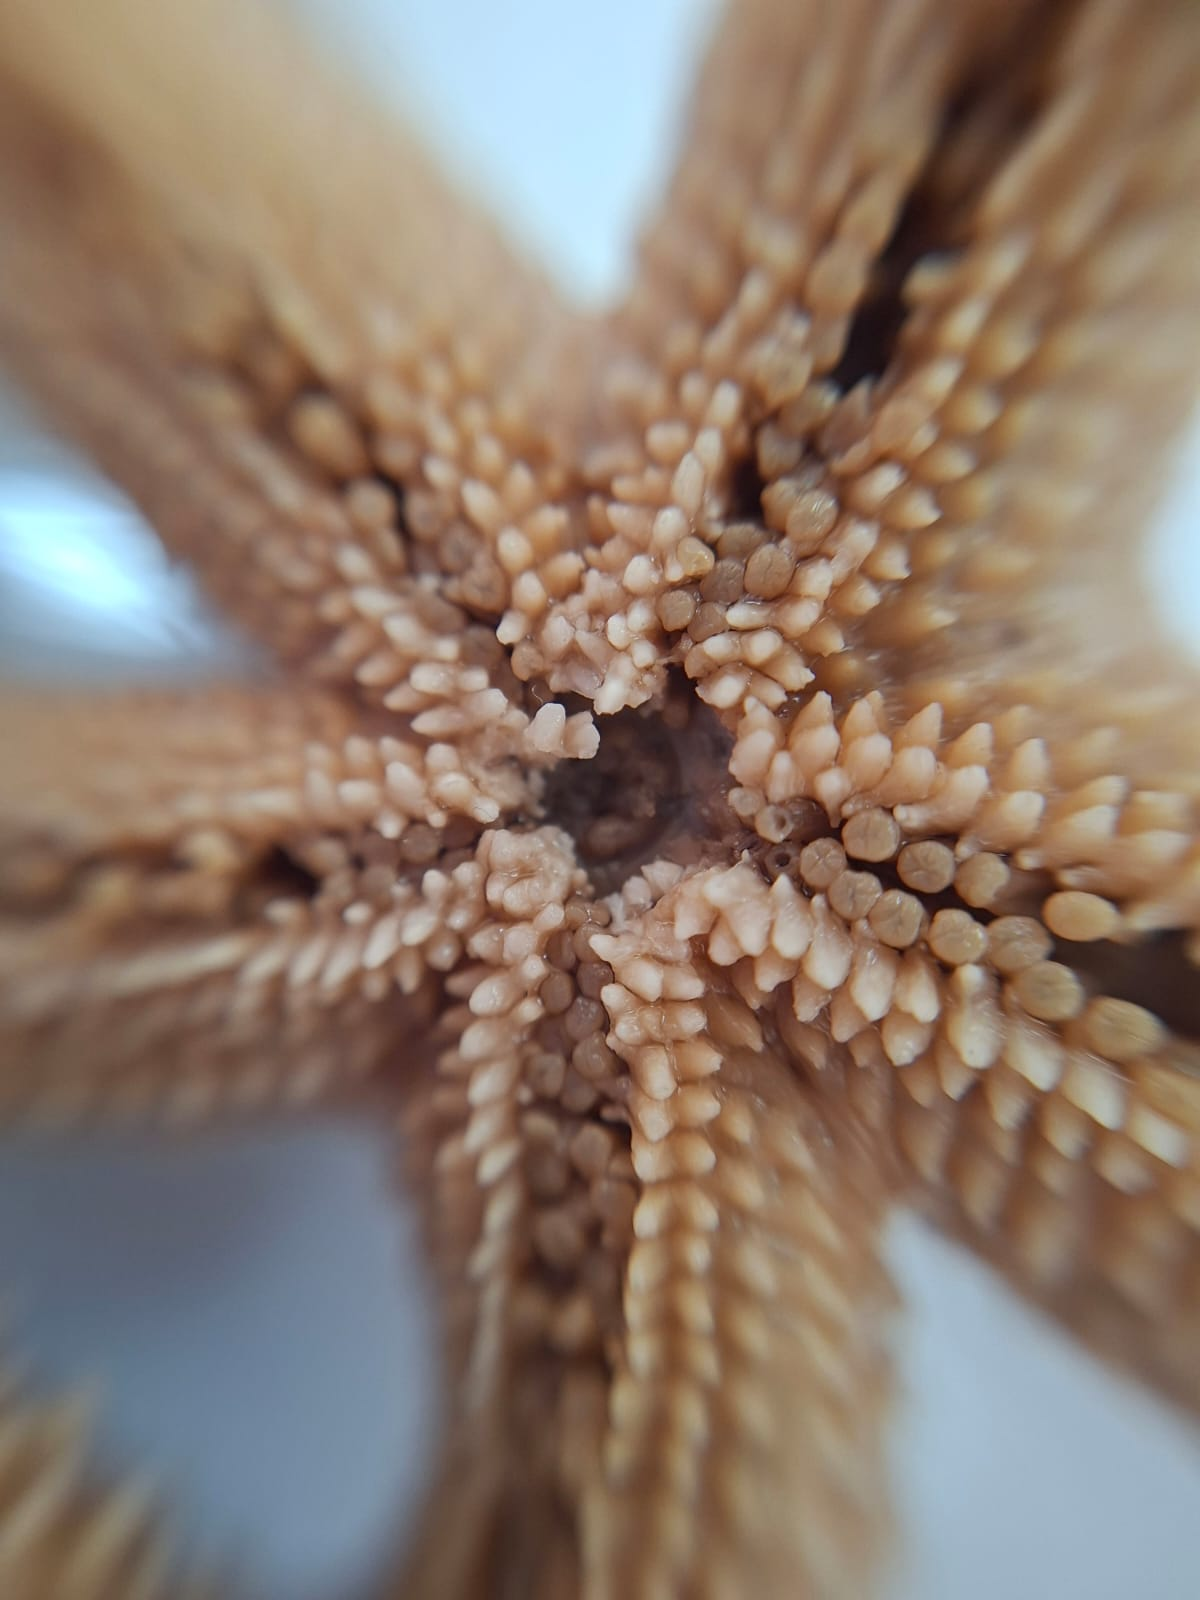
\includegraphics[width=.70\linewidth]{imagens/asteroidea_face_oral.jpg}
  \caption{Material fotográfico de aula, face oral de um asteroide. A imagem é útil para procurar a região central oral e as fileiras de pés ambulacrais associadas aos sulcos ambulacrais dos braços.}
  \label{fig:asteroidea-oral}
\end{figure}
}{}

\subsection{Ophiuroidea — serpentes-do-mar}

Características diagnósticas:

\begin{itemize}
  \item cinco braços claramente separados do disco central;
  \item braços sustentados por elementos esqueléticos articulados descritos no material como vértebras esqueléticas;
  \item pés ambulacrais sem ventosas;
  \item trato digestivo incompleto;
  \item ânus ausente;
  \item madreporito na superfície oral;
  \item locomoção principalmente pelo movimento dos braços.
\end{itemize}

O material complementar cita hábitos necrófagos, filtradores ou sedimentívoros.

\begin{pontoprova}
\textbf{Asteroidea x Ophiuroidea:} observe a transição disco--braços. Em Asteroidea, os braços continuam gradualmente a partir do disco. Em Ophiuroidea, o disco é nitidamente delimitado e os braços são finos e articulados.
\end{pontoprova}

\subsection{Echinoidea — ouriços e bolachas-do-mar}

O material distingue equinoides regulares e irregulares e apresenta:

\begin{itemize}
  \item corpo globoso ou em forma de disco;
  \item placas esqueléticas unidas, formando a testa rígida;
  \item sistema ambulacral interno à carapaça;
  \item ambúlacros fechados;
  \item aparelho mastigador interno denominado \termo{lanterna de Aristóteles};
  \item espinhos móveis, que também podem participar da locomoção.
\end{itemize}

O material complementar associa a lanterna de Aristóteles a cinco dentes calcários e apresenta algas e detritos como alimentos importantes para o grupo.

\subsection{Holothuroidea — pepinos-do-mar}

Características diagnósticas:

\begin{itemize}
  \item corpo carnoso e alongado no eixo oral--aboral;
  \item esqueleto reduzido a ossículos isolados;
  \item simetria pentâmera modificada em alguns representantes;
  \item madreporito interno;
  \item coroa de tentáculos alimentares ao redor da boca;
  \item árvore respiratória;
  \item túbulos de Cuvier em formas que os possuem;
  \item grande capacidade de evisceração e regeneração.
\end{itemize}

O material complementar caracteriza a maioria como detritívora ou suspensívora.

\IfFileExists{imagens/holothuroidea_tentaculos_1.jpg}{
\begin{figure}[H]
  \centering
  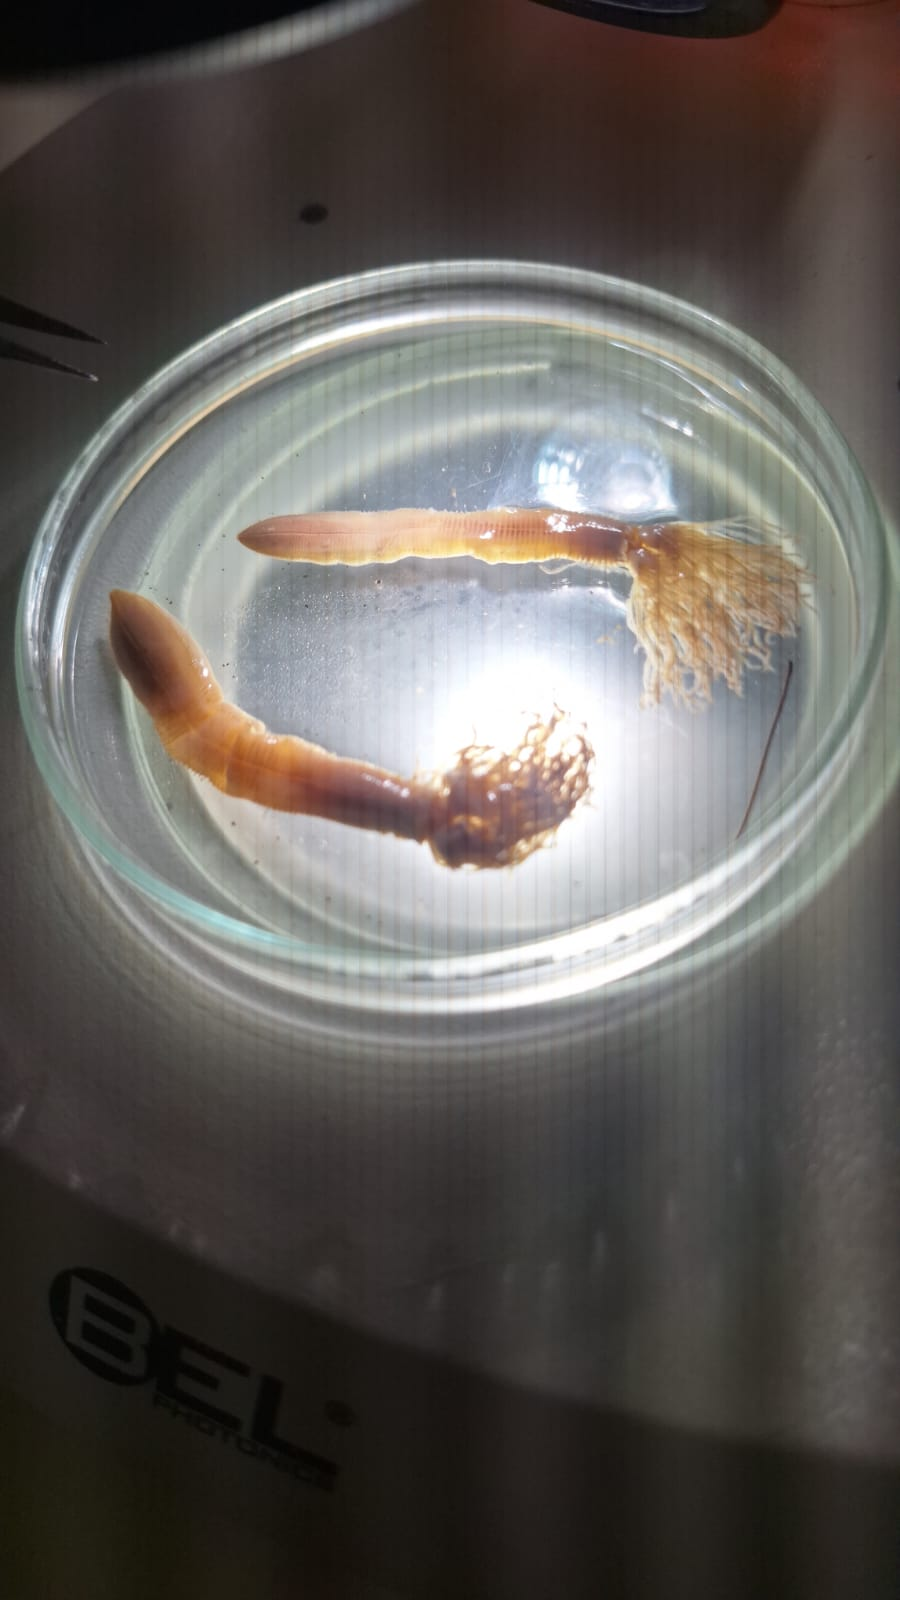
\includegraphics[width=.66\linewidth]{imagens/holothuroidea_tentaculos_1.jpg}
  \caption{Material fotográfico de aula: exemplar compatível com Holothuroidea, mostrando uma extremidade com tentáculos alimentares ao redor da boca. A identificação em nível de espécie não é feita aqui.}
  \label{fig:holothuroidea-tentaculos}
\end{figure}
}{}

\IfFileExists{imagens/holothuroidea_disseccao.jpg}{
\begin{figure}[H]
  \centering
  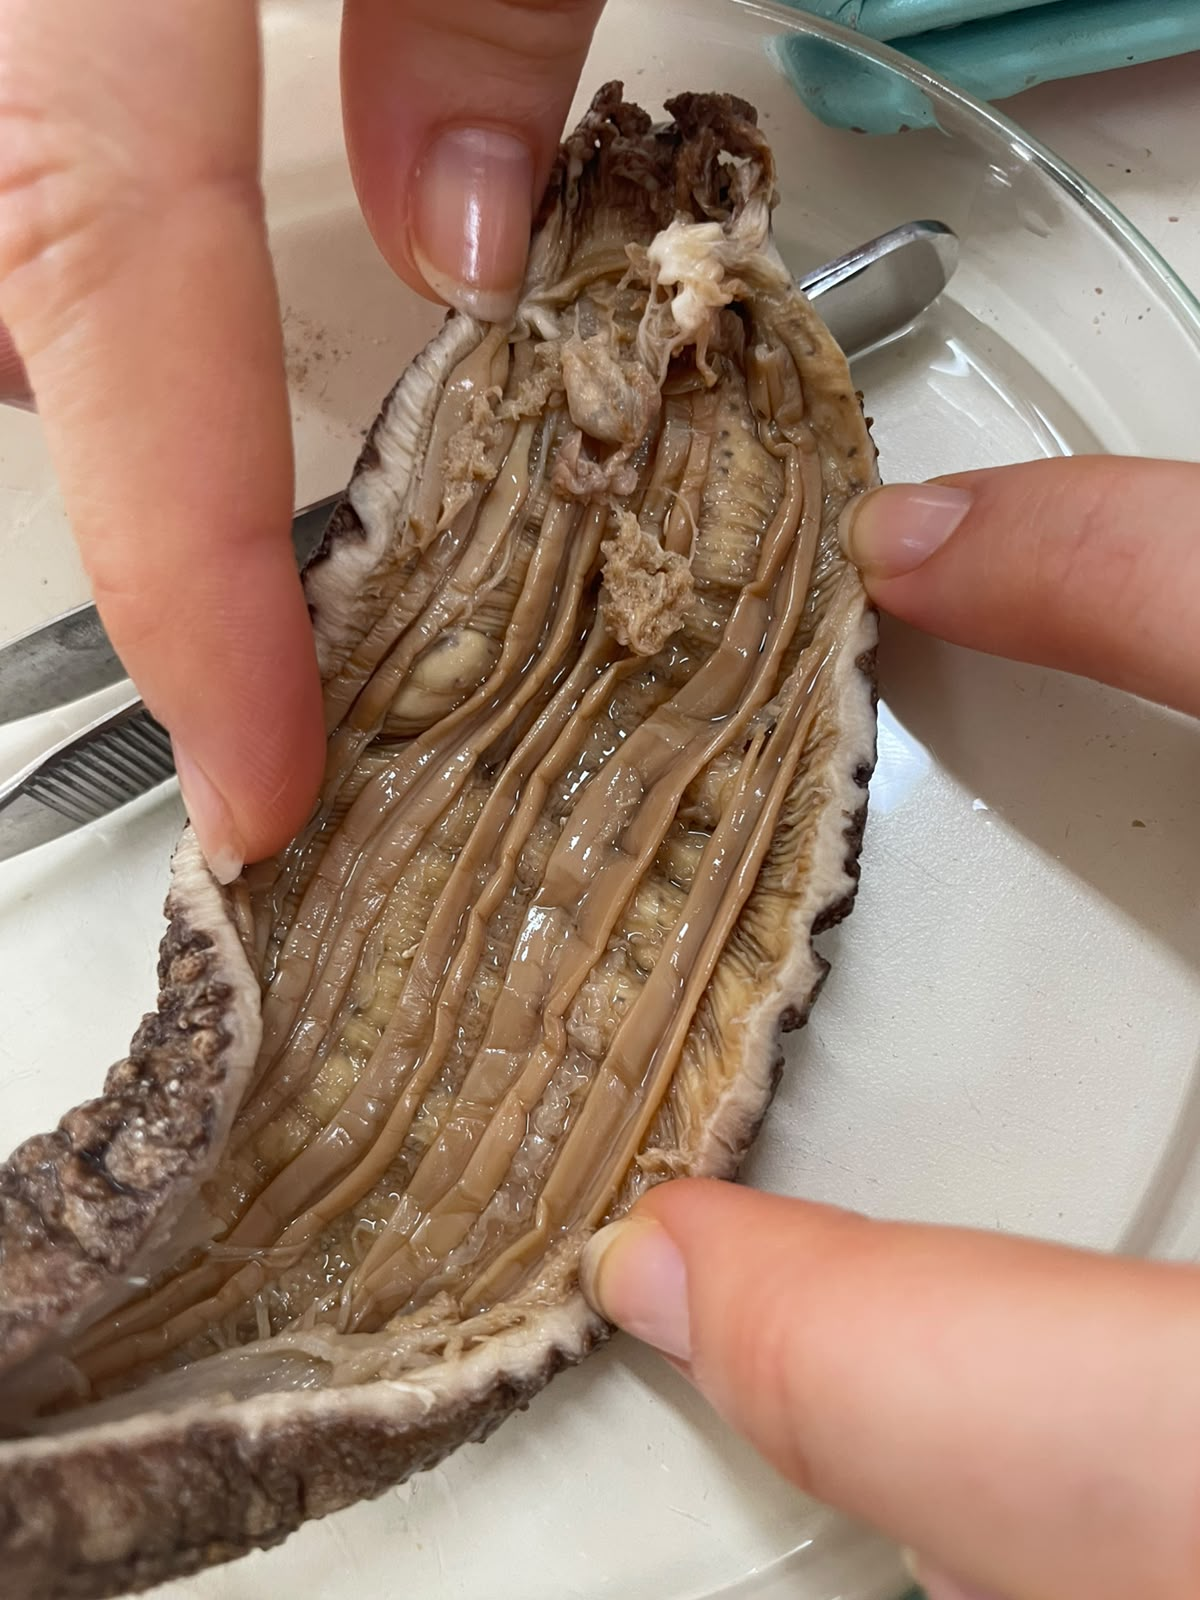
\includegraphics[width=.72\linewidth]{imagens/holothuroidea_disseccao.jpg}
  \caption{Material fotográfico de dissecção de um equinodermo alongado, compatível com Holothuroidea. A fotografia deve ser usada para relacionar a morfologia interna observada em aula às estruturas discutidas no roteiro e nos slides, sem forçar identificação de detalhes não confirmados.}
  \label{fig:holothuroidea-disseccao}
\end{figure}
}{}

% =========================================================
\section{Quadro comparativo das classes de Echinodermata}
% =========================================================

\begin{longtable}{P{2.8cm}P{3.4cm}P{3.3cm}P{3.3cm}P{3.0cm}}
\toprule
\textbf{Classe} & \textbf{Forma corporal} & \textbf{Reconhecimento} & \textbf{Sistema ambulacral / locomoção} & \textbf{Detalhe marcante} \\
\midrule
\endfirsthead
\toprule
\textbf{Classe} & \textbf{Forma corporal} & \textbf{Reconhecimento} & \textbf{Sistema ambulacral / locomoção} & \textbf{Detalhe marcante} \\
\midrule
\endhead
Crinoidea & Corpo em taça; braços ramificados & Superfície oral para cima; pínulas; pedúnculo ou cirros & Ambúlacros podem ramificar-se & Boca e ânus na superfície oral; madreporito ausente \\
Asteroidea & Corpo estrelado & Braços contínuos com o disco & Pés ambulacrais nos sulcos abertos & Madreporito e ânus aborais \\
Ophiuroidea & Disco + braços finos & Disco muito bem delimitado & Movimento principalmente pelos braços & Sem ânus; madreporito oral \\
Echinoidea & Globoso ou discoide & Testa rígida e espinhos & Pés ambulacrais + espinhos móveis & Lanterna de Aristóteles \\
Holothuroidea & Alongado e carnoso & Tentáculos ao redor da boca; ossículos reduzidos & Pés ambulacrais variáveis & Árvore respiratória; evisceração; madreporito interno \\
\bottomrule
\end{longtable}

% =========================================================
\section{Roteiro rápido de identificação prática}
% =========================================================

\begin{enumerate}
  \item \textbf{O animal é segmentado em anéis verdadeiros?}
  \begin{itemize}
    \item Se sim, pense primeiro em Annelida.
    \item Procure parapódios, cerdas, clitelo ou ventosas.
  \end{itemize}

  \item \textbf{Há parapódios laterais bem desenvolvidos?}
  \begin{itemize}
    \item Sim: Polychaeta é a principal hipótese dentro do material estudado.
    \item Parapódio birreme: procure notopódio e neuropódio.
  \end{itemize}

  \item \textbf{Há clitelo e poucas cerdas, sem parapódios?}
  \begin{itemize}
    \item Caracteres compatíveis com Oligochaeta.
  \end{itemize}

  \item \textbf{Há ventosas e numerosas anelações externas secundárias?}
  \begin{itemize}
    \item Caracteres compatíveis com Hirudinoidea.
  \end{itemize}

  \item \textbf{É um equinodermo com braços?}
  \begin{itemize}
    \item Braços contínuos com o disco: Asteroidea.
    \item Disco nitidamente separado de braços finos: Ophiuroidea.
    \item Muitos ramos/pínulas e superfície oral voltada para cima: Crinoidea.
  \end{itemize}

  \item \textbf{É um equinodermo sem braços evidentes?}
  \begin{itemize}
    \item Corpo rígido globoso/discoide com espinhos: Echinoidea.
    \item Corpo carnoso alongado com tentáculos orais: Holothuroidea.
  \end{itemize}
\end{enumerate}

% =========================================================
\section{Questões de revisão}
% =========================================================

\subsection*{Annelida}

\begin{enumerate}
  \item Quais são as três regiões corporais gerais apresentadas para Annelida?
  \item Explique por que o celoma segmentado pode funcionar como esqueleto hidrostático.
  \item Diferencie prostômio, peristômio e pigídio.
  \item Qual é a diferença entre notopódio e neuropódio?
  \item O que é um acículo e qual é sua função?
  \item Quais estruturas ajudam a reconhecer um nereidídeo em uma prática?
  \item Quais modificações caracterizam os sabelídeos tubícolas estudados?
  \item Compare as estratégias alimentares apresentadas para Polychaeta.
  \item O que é o clitelo e quais funções foram atribuídas a ele na aula?
  \item Explique a locomoção peristáltica de um oligoqueta relacionando musculatura e cerdas.
  \item Qual a função do papo, da moela e da tiflossole?
  \item Como ocorre a fecundação e o desenvolvimento no ciclo da minhoca estudado?
  \item Por que as anelações externas de uma sanguessuga não devem ser simplesmente contadas como segmentos verdadeiros?
  \item Quais são as duas ventosas importantes no reconhecimento de Hirudinoidea?
  \item Qual a função da hirudina?
\end{enumerate}

\subsection*{Echinodermata}

\begin{enumerate}[resume]
  \item Por que a simetria pentarradial dos equinodermos é considerada derivada?
  \item Diferencie a simetria da larva e do adulto.
  \item O que é estereoma?
  \item Compare o esqueleto de Echinoidea e Holothuroidea.
  \item Escreva, na ordem, os componentes principais do sistema ambulacral estudado.
  \item Por que os pés ambulacrais não devem ser considerados estruturas exclusivamente locomotoras?
  \item Diferencie Asteroidea de Ophiuroidea pela relação entre disco e braços.
  \item Em qual superfície se encontra o madreporito de Asteroidea? E de Ophiuroidea?
  \item Qual classe não possui ânus no material estudado?
  \item Qual classe possui lanterna de Aristóteles?
  \item Qual classe possui árvore respiratória?
  \item O que é evisceração e em qual classe ela foi destacada?
  \item Em Crinoidea, onde estão boca e ânus?
  \item Monte uma chave simples para separar as cinco classes apenas pela morfologia externa.
\end{enumerate}

% =========================================================
\section{Gabarito comentado — síntese}
% =========================================================

\begin{enumerate}
  \item Prostômio, tronco segmentado e pigídio.
  \item O fluido celômico oferece resistência às contrações musculares, permitindo alteração controlada da forma dos segmentos.
  \item Prostômio = região anterior; peristômio = região associada à boca; pigídio = extremidade posterior.
  \item Notopódio é o ramo dorsal; neuropódio, o ramo ventral do parapódio birreme.
  \item Acículo é uma estrutura interna de sustentação do parapódio.
  \item Prostômio desenvolvido, olhos, palpos, antenas, cirros peristomiais, probóscide eversível, paragnatas/mandíbulas e parapódios.
  \item Redução dos parapódios, ausência de acículo no exemplo, vida em tubo e coroa tentacular com radíolos; presença de uncini.
  \item O material inclui depositívoros/detritívoros, suspensívoros, predadores e parasitas.
  \item O clitelo secreta muco, albumina e participa da formação do casulo.
  \item Ondas de contração da musculatura circular e longitudinal alteram o formato dos segmentos; as cerdas alternam fixação e liberação do substrato.
  \item Papo: armazenamento; moela: trituração; tiflossole: aumento da superfície de absorção.
  \item Transferência de espermatozoides durante a cópula; fecundação externa no interior do casulo; desenvolvimento direto.
  \item Porque há anelações secundárias externas além da segmentação primária.
  \item Ventosas anterior e posterior.
  \item Anticoagulante produzido por glândulas salivares de formas hematófagas.
  \item Porque as larvas são bilaterais e a pentarradialidade do adulto foi adquirida secundariamente.
  \item Larva bilateral; adulto radial pentâmero.
  \item Rede porosa característica dos elementos calcários do endoesqueleto.
  \item Echinoidea: ossículos fortemente unidos formando testa; Holothuroidea: ossículos reduzidos e isolados na derme.
  \item Madreporito $\rightarrow$ canal pétreo $\rightarrow$ canal circular $\rightarrow$ canais radiais $\rightarrow$ ampolas $\rightarrow$ pés ambulacrais.
  \item Porque também podem participar de fixação, alimentação, percepção e trocas gasosas.
  \item Asteroidea: braços contínuos com o disco; Ophiuroidea: disco claramente separado dos braços.
  \item Asteroidea: aboral; Ophiuroidea: oral.
  \item Ophiuroidea.
  \item Echinoidea.
  \item Holothuroidea.
  \item Eliminação de partes internas, seguida de regeneração; destacada em Holothuroidea.
  \item Ambos na superfície oral.
  \item Resposta deve usar: braços/disco, forma rígida globosa ou discoide, forma alongada, pínulas/pedúnculo, tentáculos orais e relação disco--braços.
\end{enumerate}

% =========================================================
\section{Material-base desta versão}
% =========================================================

Esta versão foi construída exclusivamente a partir dos materiais fornecidos para estudo:

\begin{itemize}
  \item \textit{01 Annelida Polychaeta.pdf} — aula de Annelida/Polychaeta;
  \item \textit{02 Oligochaeta e Hirudinea.pdf} — aula de Clitellata, Oligochaeta e Hirudinoidea;
  \item \textit{pratica-annelida (1).pdf} — roteiro de morfologia externa e prática de Annelida;
  \item \textit{Aula\_Echinodermata\_Mariana Contins.pdf} — aula teórica de Echinodermata;
  \item \textit{equinodermos.pdf} — material complementar fornecido;
  \item fotografias fornecidas pelo aluno para revisão da prática.
\end{itemize}

\begin{atencao}
A seção de Lofoforados ainda não foi preenchida. Ela deve ser incorporada a partir do material específico da disciplina, sem extrapolar o conteúdo ministrado.
\end{atencao}

\end{document}
